% ============================================================
%  FICHIER MAÎTRE — Projet Environnement
%  CY Cergy Paris Université — L2 Informatique
% ============================================================
\documentclass[12pt, a4paper]{article}

% --- Encodage et langue ---
\usepackage[utf8]{inputenc}
\usepackage[T1]{fontenc}
\usepackage[french]{babel}

% --- Correction headheight (warning fancyhdr) ---
\setlength{\headheight}{15.5pt}

% --- Mise en page ---
\usepackage[top=2.5cm, bottom=2.5cm, left=3cm, right=2.5cm]{geometry}
\usepackage{fancyhdr}
\usepackage{emptypage}
\usepackage{setspace}
\usepackage{etoolbox}
\usepackage{needspace}

% --- Typographie ---
\usepackage{microtype}
\usepackage{lmodern}
\setlength{\parskip}{0.5\baselineskip}
\setlength{\parindent}{1.5em}
\onehalfspacing
% Correction des débordements de texte (Overfull \hbox)
\emergencystretch=2em

% --- Graphiques et couleurs ---
\usepackage{graphicx}
\usepackage[dvipsnames, table]{xcolor}
\graphicspath{{images/}}
\usepackage{float}
\usepackage{caption}
\usepackage{subcaption}

% --- Mathématiques ---
\usepackage{amsmath}
\usepackage{amssymb}

% --- Tableaux ---
\usepackage{booktabs}
\usepackage{tabularx}
\usepackage{multirow}
\usepackage{array}
\usepackage{longtable}

% --- Listes ---
\usepackage{enumitem}
\setlist[itemize]{noitemsep, topsep=0.3em}
\setlist[enumerate]{noitemsep, topsep=0.3em}

% --- Code source ---
\usepackage{listings}
\definecolor{codebg}{RGB}{248, 248, 248}
\definecolor{codeframe}{RGB}{180, 180, 180}
\definecolor{codekw}{RGB}{0, 0, 180}
\definecolor{codecomment}{RGB}{80, 120, 80}
% Couleur chaînes : brun-orangé (pas rouge)
\definecolor{codestring}{RGB}{150, 80, 0}

\lstdefinestyle{java}{
  language=Java,
  backgroundcolor=\color{codebg},
  frame=single,
  rulecolor=\color{codeframe},
  basicstyle=\ttfamily\footnotesize,
  keywordstyle=\bfseries\color{codekw},
  commentstyle=\itshape\color{codecomment},
  stringstyle=\color{codestring},
  numbers=left,
  numberstyle=\tiny\color{gray},
  numbersep=8pt,
  stepnumber=1,
  breaklines=true,
  breakatwhitespace=true,
  captionpos=b,
  tabsize=4,
  showstringspaces=false,
  extendedchars=true,
  literate=
    {é}{{\'e}}1 {è}{{\`e}}1 {ê}{{\^e}}1 {à}{{\`a}}1
    {ù}{{\`u}}1 {ô}{{\^o}}1 {î}{{\^i}}1 {û}{{\^u}}1
    {â}{{\^a}}1 {ç}{{\c{c}}}1 {É}{{\'E}}1 {È}{{\`E}}1
    {Ê}{{\^E}}1 {À}{{\`A}}1
}

\lstdefinestyle{algo}{
  backgroundcolor=\color{codebg},
  frame=single,
  rulecolor=\color{codeframe},
  basicstyle=\ttfamily\footnotesize,
  keywordstyle=\bfseries,
  numbers=left,
  numberstyle=\tiny\color{gray},
  numbersep=8pt,
  stepnumber=1,
  breaklines=true,
  captionpos=b,
  tabsize=2,
  extendedchars=true,
  literate=
    {é}{{\'e}}1 {è}{{\`e}}1 {ê}{{\^e}}1 {à}{{\`a}}1
    {ù}{{\`u}}1 {ô}{{\^o}}1 {î}{{\^i}}1 {û}{{\^u}}1
    {â}{{\^a}}1 {ç}{{\c{c}}}1 {É}{{\'E}}1
}

% --- Hyperliens ---
\usepackage[hidelinks, hypertexnames=false]{hyperref}
\usepackage{url}

% --- Formatage des titres ---
\usepackage{titlesec}
\titleformat{\section}{\Large\bfseries}{\thesection}{1em}{}[\vspace{0.3em}\hrule\vspace{0.5em}]
\titleformat{\subsection}{\large\bfseries}{\thesubsection}{1em}{}
\titlespacing*{\section}{0pt}{2em}{1em}
\titlespacing*{\subsection}{0pt}{1.5em}{0.5em}
\pretocmd{\section}{\clearpage}{}{}   

% Numérotation des sections
\setcounter{secnumdepth}{2}
\setcounter{tocdepth}{2}

% --- En-têtes et pieds de page ---
\pagestyle{fancy}
\fancyhf{}
\renewcommand{\headrulewidth}{0.4pt}
\renewcommand{\footrulewidth}{0.2pt}
\fancyhead[L]{\slshape\leftmark}
\fancyhead[R]{\thepage}
\fancyfoot[C]{\small Projet Environnement~---~CY Cergy Paris Université~---~Année 2025--2026}

% Page de style plain (table des matières, etc.)
\fancypagestyle{plain}{%
  \fancyhf{}
  \fancyfoot[C]{\thepage}
  \renewcommand{\headrulewidth}{0pt}
}

% ============================================================
\begin{document}
% ============================================================

% --- Page de garde ---
% ============================================================
%  PAGE DE GARDE — titre.tex
% ============================================================
\begin{titlepage}
  \centering

  % --- Bandeau supérieur ---
  \begin{minipage}[t]{0.45\textwidth}
    \raggedright
    
\includegraphics[height=2cm]{images/logo_universite.png}
  \end{minipage}
  \hfill
  \begin{minipage}[t]{0.45\textwidth}
    \raggedleft
    \textsc{\small CY Cergy Paris Université}\\[0.2em]
    \small UFR Sciences et Techniques\\
    \small Département Informatique
  \end{minipage}

  \vspace{0.5cm}
  \hrule height 0.8pt
  \vspace{0.5cm}

  % --- Mention du cursus ---
  {\large\textsc{Licence 2 Informatique}}\\[0.3em]
  {\normalsize Génie Logiciel et Conception de Logiciels}\\[0.5em]
  {\large\bfseries RAPPORT DE PROJET}

  \vspace{1.5cm}

  % --- Image décorative ---
  \begin{center}
    \fbox{%
      \begin{minipage}{0.4\textwidth}
        \centering
        \vspace{0.2cm}
        
\includegraphics[width=0.35\textwidth]{images/logo.png}
        \vspace{0.2cm}
      \end{minipage}%
    }
  \end{center}

  \vspace{0.2cm}

  % --- Titre du projet ---
  {\Huge\bfseries Simulateur d'Écosystème}\\[0.5em]
  {\LARGE\bfseries Dynamique en Java}

  \vspace{0.4cm}
  \hrule height 0.4pt
  \vspace{0.4cm}

  {\large\itshape Conception et implémentation d'un simulateur}\\
  {\large\itshape d'évolution de biomes géré par événements}

  \vspace{2cm}

  % --- Auteurs ---
  \begin{minipage}{0.6\textwidth}
    \centering
    \large
    \begin{tabular}{l}
      \scshape{Feraoun} Mohamed Amine\\[0.4em]
      \scshape{Anurajan} Thenuxshan\\[0.4em]
      \scshape{Ouardani} Nidhal
    \end{tabular}
  \end{minipage}

  \vfill

  % --- Encadrant et date ---
  \begin{minipage}{0.48\textwidth}
    \raggedright
    \textbf{Encadrant~:}\\[0.3em]
    \underline{Tianxiao LIU}\\
    
  \end{minipage}
  \hfill
  \begin{minipage}{0.48\textwidth}
    \raggedleft
    \textbf{Année universitaire~:}\\[0.3em]
    2025 -- 2026\\[0.5em]
    \textbf{Date de dépôt~:} Avril 2026
  \end{minipage}

  \vspace{0.2cm}
  \hrule height 0.8pt

\end{titlepage}

% --- Table des matières ---
\tableofcontents
\clearpage

% --- Liste des figures ---
\listoffigures
\clearpage

% --- Liste des tableaux ---
\listoftables
\clearpage

% --- Remerciements ---
% ============================================================
%  REMERCIEMENTS — remerciements.tex
% ============================================================
\clearpage
\thispagestyle{empty}

\vspace*{2cm}

\begin{center}
{\LARGE\bfseries Remerciements du groupe}
\end{center}

\vspace{2cm}

\begin{flushleft}

 Nous tenons à exprimer notre profonde gratitude envers toutes les personnes qui ont contribué, de près ou de loin, à la réalisation de ce projet.

\vspace{1.5cm}

Nos remerciements s'adressent en premier lieu à notre professeur encadrant, M. Tianxiao LIU, pour ses précieux conseils, son suivi régulier et son accompagnement tout au long de ce projet. Ses orientations méthodologiques et techniques ont été déterminantes dans l'aboutissement de ce travail.

\vspace{1cm}

Nous remercions également l'UFR Sciences et Techniques de CY Cergy Paris Université pour les ressources mises à disposition et l'environnement propice à l'apprentissage qu'elle a su créer. Les enseignements dispensés au sein de la Licence 2 Informatique ont constitué le socle indispensable à la réalisation de ce simulateur.

\vspace{1cm}

Nos remerciements vont aussi à nos pairs pour les échanges constructifs et les réflexions partagées qui ont enrichi notre compréhension des concepts abordés.

\end{flushleft}

\vspace{2cm}
\clearpage

% --- Corps du rapport ---
% ============================================================
%  INTRODUCTION — introduction.tex
% ============================================================
\section{Introduction}
\label{sec:introduction}

Le projet \textbf{Environnement} est une application de simulation écologique
développée en Java~8. Une simulation écologique est un modèle informatique qui
reproduit l'évolution d'un écosystème naturel au cours du temps, permettant
d'étudier les interactions entre différents éléments et leur milieu. L'écosystème
simulé est représenté par une grille où chaque cellule contient un \emph{biome},
c'est-à-dire une région naturelle caractérisée par son climat et sa végétation.
Sept types de biomes sont modélisés~: Forêt, Désert, Mer, Montagne, Banquise,
Ville et Village. Chaque biome possède des propriétés intrinsèques (température,
humidité, pollution, purification) qui définissent son état environnemental à
un instant donné.

\begin{figure}[htbp]
  \centering
  
\includegraphics[width=0.25\textwidth]{images/logo.png}
  \caption{Logo du projet Environnement}
  \label{fig:logo_projet}
\end{figure}

La dimension temporelle de la simulation est structurée par des \emph{rounds}.
À chaque round, des événements météorologiques (Pluie, Vent, Pollution, Météore,
entre autres) affectent les caractéristiques des biomes et peuvent déclencher
des transformations automatiques selon des règles écologiques prédéfinies. Par
exemple, une forêt soumise à une longue période de sécheresse peut se transformer
en désert.

\subsection{Problématique du projet}
\label{subsec:problematique}

La problématique centrale consiste à concevoir un système de simulation permettant
de gérer l'évolution dynamique d'un écosystème sur une grille bidimensionnelle,
dans la tradition des automates cellulaires popularisés par Conway~\cite{gardner1970life}.
Plusieurs questions ont guidé le développement~: comment un biome réagit-il aux
conditions environnementales changeantes telles que la température, l'humidité et
la pollution~? Comment les événements climatiques propagent-ils leurs effets sur
la carte~? Quand et selon quelles conditions un biome se transforme-t-il en un
autre type~? Comment visualiser cette évolution de manière fluide et interactive
sur une interface graphique~?
\needspace{1\baselineskip}
Ces questions convergent vers un objectif synthétique~: créer une simulation
dynamique et réaliste, accessible et pilotable via une interface graphique
développée avec la bibliothèque Java Swing.

\subsection{Enjeux de la conception logicielle}
\label{subsec:enjeux}

Ce projet présente plusieurs enjeux majeurs sur le plan de la conception logicielle.
Les enjeux identifiés sont les suivants: 

\begin{itemize}
  \item \textbf{Extensibilité}~: l'architecture doit permettre l'ajout de nouveaux
    types de biomes ou d'événements sans modifier le code existant, ce qui implique
    une séparation rigoureuse entre les données et les traitements.
  \item \textbf{Maintenabilité}~: le code doit être modulaire et bien structuré
    pour faciliter les évolutions futures et la correction d'anomalies.
  \item \textbf{Travail collaboratif}~: en équipe de trois développeurs, des
    conventions partagées et une conception claire sont indispensables pour garantir
    la cohérence du code et éviter les conflits.
  \item \textbf{Modélisation réaliste}~: les règles de transformation écologique
    doivent refléter des phénomènes naturels plausibles tout en restant
    implémentables dans les contraintes du projet.
\end{itemize}

\subsection{Objectifs du projet}
\label{subsec:objectifs}

L'objectif principal est de développer une application complète de simulation
écologique reposant sur quatre fonctionnalités fondamentales~:

\begin{itemize}
  \item la création d'une carte configurable composée de sept types de biomes
    (Forêt, Désert, Mer, Montagne, Banquise, Ville, Village)~;
  \item l'apparition dynamique d'événements environnementaux (Pluie, VentFroid,
    VentChaud, Pollution, Purification, Météore et leurs variantes)~;
  \item la transformation automatique des biomes selon six règles écologiques~:
    Inondation, Glaciation, Désertification, Forestation, Civilisation
    et Densification~;
  \item la visualisation en temps réel via une interface graphique interactive
    développée avec Java Swing.
\end{itemize}
\needspace{5\baselineskip}
Plusieurs fonctionnalités secondaires ont également été intégrées~: une fenêtre de
statistiques en temps réel avec des graphiques d'évolution générés par la
bibliothèque JFreeChart, un mode édition interactif, une fenêtre de tutoriel
permettant la prise en main rapide de l'application, ainsi qu'une option de
contrôle de la vitesse de simulation.

\subsection{Organisation du rapport}
\label{subsec:organisation}

Ce rapport est structuré en six sections principales qui couvrent l'ensemble du
cycle de vie du projet~\cite{wikibooks2024latex}. La section~\ref{sec:specification} établit le référentiel
fonctionnel~: fonctionnalités attendues, terminologie, contraintes techniques et
règles de comportement du simulateur. La section~\ref{sec:realisation} détaille
la conception logicielle et sa mise en œuvre~: architecture modulaire, hiérarchie
des classes, design patterns appliqués à notre code et traitements
algorithmiques au cœur du moteur. Le manuel d'installation et d'utilisation,
constituant un guide opérationnel destiné à tout utilisateur souhaitant prendre
en main l'application, est proposé à la section~\ref{sec:manuel}. La
section~\ref{sec:deroulement} retrace le déroulement concret du projet~:
organisation de l'équipe, phases de développement, outils employés et difficultés
techniques surmontées. Enfin, la section~\ref{sec:conclusion} dresse le bilan du
travail accompli et propose des perspectives d'amélioration pour les versions
futures du simulateur.

% ============================================================
%  SPÉCIFICATION — specification.tex
% ============================================================
\section{Spécification du simulateur}
\label{sec:specification}

Cette section détaille les fonctionnalités attendues du projet ainsi que les
contraintes qui définissent son comportement. Elle constitue le référentiel
fonctionnel sur lequel s'appuie la conception décrite dans la
section~\ref{sec:realisation}.

% ------------------------------------------------------------
\subsection{Notions de base et contraintes du projet}
\label{subsec:notions_base}

Cette sous-section définit les fondements du modèle de simulation, établit le
vocabulaire technique utilisé dans l'ensemble du rapport et recense les
limitations connues de l'application.

\paragraph{Fonctionnement général du logiciel.}
Le fonctionnement repose sur un modèle de simulation par \emph{rounds} successifs.
À chaque round, le système exécute un cycle complet divisé en quatre étapes
distinctes, comme l'illustre la figure~\ref{fig:flux_round}.

\begin{figure}[H]
  \centering
  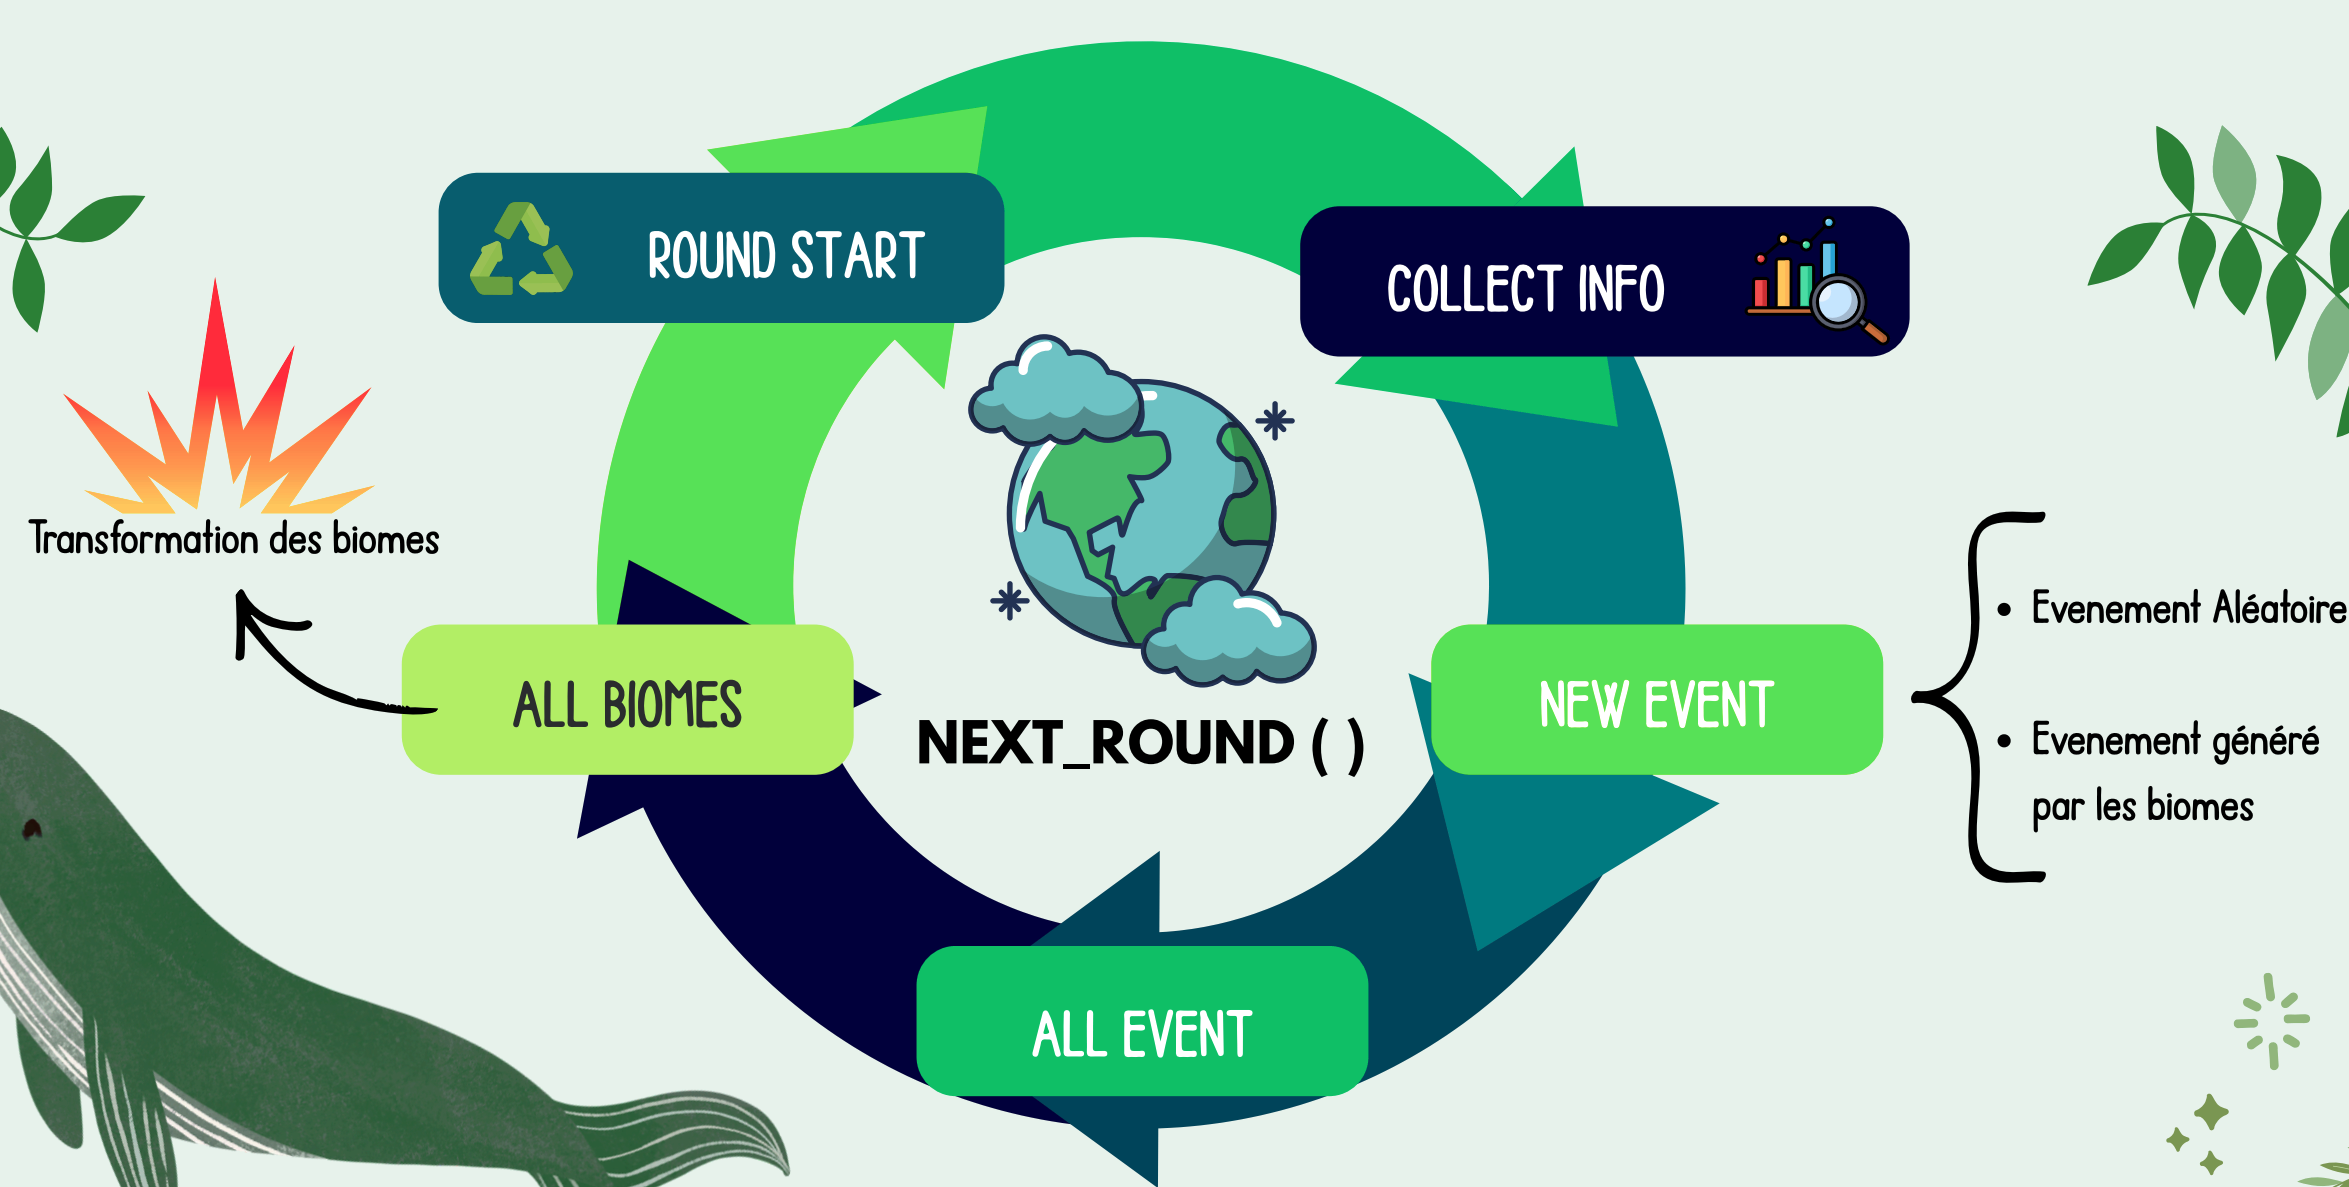
\includegraphics[width=0.75\textwidth]{images/flux_round.png}
  \caption{Flux d'exécution d'un round de simulation}
  \label{fig:flux_round}
\end{figure}

\begin{enumerate}
  \item \textbf{Génération d'événements}~: au début de chaque round, de nouveaux
    événements météorologiques apparaissent aléatoirement sur la carte selon des
    probabilités configurables.
  \item \textbf{Déplacement des événements}~: les événements mobiles se déplacent
    d'une case dans leur direction assignée~; ce déplacement peut être bloqué par
    les biomes Montagne.
  \item \textbf{Application des impacts}~: les événements modifient les propriétés
    numériques des biomes qu'ils occupent.
  \item \textbf{Évaluation des transformations}~: les règles de transformation
    vérifient les propriétés de chaque biome~; si les conditions sont satisfaites,
    le biome se transforme en un autre type.
\end{enumerate}

La carte est représentée par une grille bidimensionnelle configurable dont chaque
cellule contient exactement un biome. Chaque biome possède quatre propriétés
numériques bornées entre~0 et~100~: température, humidité, pollution et
purification.

\paragraph{Vocabulaire et terminologies de base.}
Les termes techniques récurrents dans ce rapport sont définis comme suit.

\begin{itemize}
  \item \textbf{Biome}~: unité de base de la carte représentant un type
    d'écosystème distinct (Forêt, Désert, Mer, Montagne, Banquise, Ville,
    Village).
  \item \textbf{Round}~: cycle d'exécution de la simulation comprenant les quatre
    étapes de génération, déplacement, impact et transformation.
  \item \textbf{Événement}~: phénomène météorologique affectant les propriétés
    numériques des biomes (Pluie, VentFroid, VentChaud, Pollution, etc.).
  \item \textbf{Transformation}~: changement automatique d'un biome vers un autre
    type selon les règles écologiques définies.
  \item \textbf{Carte}~: grille bidimensionnelle de blocs, chaque bloc contenant
    un biome identifié par ses coordonnées $(x, y)$.
  \item \textbf{Propriétés}~: les quatre caractéristiques numériques d'un biome,
    à savoir la température, l'humidité, la pollution et la purification.
\end{itemize}

\paragraph{Contraintes et limitations connues.}
L'application présente plusieurs contraintes et limitations identifiées lors de
son développement.

La première limitation concerne l'\textbf{absence de persistance des données}.
L'état de l'écosystème est intégralement géré en mémoire vive durant l'exécution.
Le logiciel ne dispose pas de mécanisme de sérialisation permettant de sauvegarder
l'état d'une simulation pour la reprendre ultérieurement.

La deuxième limitation porte sur les \textbf{contraintes de l'interface
Homme-Machine}. L'interface graphique possède une résolution fixée à
1920\,$\times$\,1080~pixels. Le positionnement absolu des composants Swing empêche
un redimensionnement dynamique de la fenêtre, et l'ergonomie du mode édition ne
prend pas en charge la sélection de masse ni la duplication de zones.

La troisième limitation concerne le \textbf{couplage entre le moteur et
l'interface graphique}. Le gestionnaire de simulation (\texttt{ManageurBasique})
communique directement avec certains composants Swing, ce qui crée une dépendance
bidirectionnelle entre la logique métier et la couche de présentation. Ce couplage
rend le remplacement ou le test isolé du moteur plus complexe qu'avec une
architecture entièrement découplée.

La quatrième limitation est l'\textbf{absence de parallélisme dans le moteur de
simulation}. Toutes les étapes d'un round~--- génération, déplacement, impact et
transformation~--- s'exécutent séquentiellement dans un unique thread. Sur des
cartes de grande taille ou avec un nombre d'entités élevé, cette approche
séquentielle constitue un goulot d'étranglement, car les interactions entre
événements et biomes ne tirent aucun parti du multi-cœur du processeur.

% ------------------------------------------------------------
\subsection{Fonctionnalités attendues du projet}
\label{subsec:fonctionnalites}

Cette sous-section recense l'ensemble des fonctionnalités que l'application doit
implémenter, organisées par domaine fonctionnel.

\paragraph{Gestion de la carte.}
La carte est représentée par une grille bidimensionnelle de cellules appelées
\emph{blocs}. Chaque bloc contient un biome et est identifié par ses coordonnées
$(x, y)$. Les dimensions de la grille sont configurables (par exemple
$20 \times 20$ ou $30 \times 30$). La figure~\ref{fig:grille_biome} montre un
exemple de grille peuplée de biomes variés.

\begin{figure}[H]
  \centering
  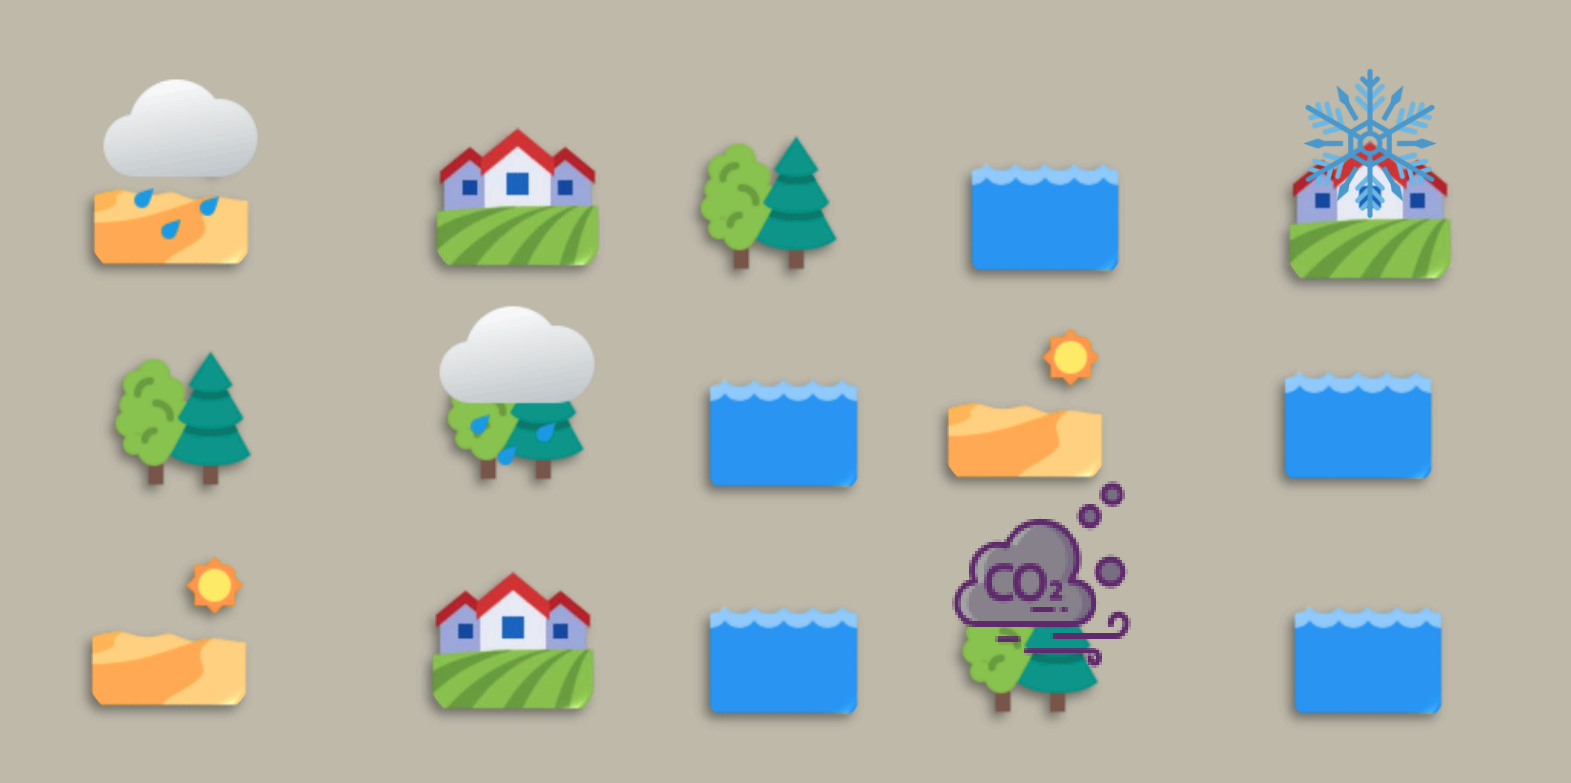
\includegraphics[width=0.7\textwidth]{images/grille_biome.png}
  \caption{Exemple de grille de biomes générée par l'application}
  \label{fig:grille_biome}
\end{figure}

La génération de la carte peut s'effectuer de manière aléatoire, les probabilités
de chaque type de biome étant définies dans le fichier de configuration. Chaque bloc
est accessible et modifiable via des méthodes d'accès dédiées. Les coordonnées sont
validées avant tout accès pour garantir la cohérence des données.

\paragraph{Gestion des biomes.}
L'application modélise sept types de biomes, chacun représentant un écosystème
distinct avec des propriétés environnementales spécifiques (température, humidité,
pollution, purification). La Montagne constitue une exception notable~: elle est
immuable et ne peut être transformée par aucune règle. Les transformations entre
biomes suivent des chaînes logiques reflétant des phénomènes écologiques
plausibles~; par exemple, une Forêt soumise à la désertification devient un Désert,
lequel peut, sous l'effet inverse de la forestation, redevenir une Forêt. Les
valeurs initiales des propriétés de chaque biome et leur hiérarchie d'implémentation
sont présentées dans la section~\ref{sec:realisation}.

\paragraph{Gestion des événements.}
L'application gère treize types d'événements divisés en deux catégories. Les
événements statiques restent à une position fixe pendant leur durée de vie~; le
Météore est le seul représentant de cette catégorie. Les événements mobiles se
déplacent d'une case à chaque round dans une direction assignée. Le
tableau~\ref{tab:evenements} synthétise les propriétés de chaque événement.

\begin{table}[H]
  \centering
  \caption{Propriétés des événements météorologiques}
  \label{tab:evenements}
  \begin{tabular}{llrrrr>{\small}r}
    \toprule
    \textbf{Événement} & \textbf{Catégorie} & \textbf{Durée}
      & $\Delta$\textbf{Temp.} & $\Delta$\textbf{Hum.}
      & $\Delta$\textbf{Poll.} & $\Delta$\textbf{Purif.} \\
    \midrule
    Pluie         & Mobile  &  4 &   0   & $+$5  &   0   &  0 \\
    VentFroid     & Mobile  &  4 & $-$5  &   0   &   0   &  0 \\
    Pollution     & Mobile  &  4 &   0   &   0   & $+$10 &  0 \\
    Purification  & Mobile  &  4 &   0   &   0   &   0   & $+$5 \\
    Météore       & Statique & 20 & $+$50 &   0   & $+$20 &  0 \\
    Orage         & Mobile  &  6 &   0   & $+$10 &   0   &  0 \\
    Grêle         & Mobile  &  3 & $-$10 & $+$5  &   0   &  0 \\
    Tornade       & Mobile  &  8 &   0   & $+$5  & $+$5  &  0 \\
    PluieBénite   & Mobile  &  5 &   0   & $+$8  & $-$5  & $+$10 \\
    Zéphyr        & Mobile  &  3 & $+$5  &   0   &   0   &  0 \\
    Tonnerre      & Mobile  &  2 &   0   & $+$8  &   0   &  0 \\
    Smog          & Mobile  &  6 &   0   &   0   & $+$15 &  0 \\
    NuageToxique  & Mobile  &  7 &   0   &   0   & $+$20 &  0 \\
    \bottomrule
  \end{tabular}
\end{table}

Comme le montre le tableau~\ref{tab:evenements}, les événements mobiles exercent
des impacts différenciés sur les quatre propriétés des biomes. Chaque événement
mobile possède une durée de vie~; à son expiration, il est retiré de la carte.
Lorsqu'un déplacement est bloqué par une Montagne, l'événement choisit une
nouvelle direction aléatoire~; s'il n'en existe aucune, il reste en place.

Chaque événement est généré selon une formation spatiale définie, lui conférant
une empreinte visuelle reconnaissable sur la grille. Le
tableau~\ref{tab:formations} détaille la formation associée à chaque type
d'événement.

\begin{table}[H]
  \centering
  \caption{Formations spatiales des événements météorologiques}
  \label{tab:formations}
  \begin{tabular}{ll}
    \toprule
    \textbf{Événement} & \textbf{Formation} \\
    \midrule
    Pluie, PluieAcide, Orage, PluieBénite & Carré 2$\times$2 \\
    VentFroid, VentChaud & Ligne horizontale \\
    Grêle & Ligne verticale \\
    Tornade & Croix \\
    Zéphyr & Diagonale \\
    Tonnerre & Forme en T \\
    Smog, NuageToxique & Cercle \\
    Pollution, Purification, Météore & Unique \\
    \bottomrule
  \end{tabular}
\end{table}

\paragraph{Système de transformation des biomes.}
Six règles de transformation écologique contrôlent l'évolution des biomes au fil
des rounds. Le tableau~\ref{tab:transformations} présente les conditions
d'activation de chaque règle et le biome cible associé.

\begin{table}[H]
  \centering
  \caption{Règles de transformation écologique et conditions d'activation}
  \label{tab:transformations}
  \begin{tabular}{llp{7cm}}
    \toprule
    \textbf{Règle} & \textbf{Biome cible} & \textbf{Condition principale} \\
    \midrule
    Inondation      & Mer      & Humidité $\geq 90$, Temp.\ $\geq 5$, Poll.\ $\leq 40$ \\
    Glaciation      & Banquise & Temp.\ $\leq 0$, Hum.\ $\geq 20$, Poll.\ $\leq 20$ \\
    Désertification & Désert   & Temp.\ $\geq 50$ ou Hum.\ $\leq 10$ \\
    Forestation     & Forêt    & Temp.\ $\in [10, 35]$, Hum.\ $\in [60, 90]$, Poll.\ $\leq 25$ \\
    Civilisation    & Village  & Temp.\ $\in [15, 40]$, Hum.\ $\in [20, 80]$, Poll.\ $\leq 10$ \\
    Densification   & Ville    & Temp.\ $\in [18, 45]$, Hum.\ $\in [30, 70]$, Poll.\ $\in [10, 60]$ \\
    \bottomrule
  \end{tabular}
\end{table}

Les conditions décrites dans le tableau~\ref{tab:transformations} sont évaluées à
chaque round pour chaque biome de la carte. Chaque règle est implémentée sous
forme d'un objet indépendant, ce qui garantit leur évaluation uniforme par le
moteur de simulation sans modification de l'algorithme principal.

\paragraph{Interface graphique.}
L'interface graphique permet de visualiser et de contrôler la simulation en temps
réel. La carte est affichée sous forme de grille colorée où chaque cellule
représente un biome distinct. Les événements sont superposés à la grille sous forme
de symboles animés. L'interface propose les contrôles suivants~: Play pour démarrer
la simulation, Pause pour la suspendre, Vitesse~$\times 2$ pour accélérer
l'exécution, Bilan de fin pour consulter le récapitulatif, et Statistiques pour
ouvrir la fenêtre d'analyse détaillée. Un mode édition permet de modifier
manuellement les biomes avant ou pendant la simulation. Une fenêtre de tutoriel
est également disponible pour guider l'utilisateur lors de sa première utilisation.

% ============================================================
%  CONCEPTION ET MISE EN ŒUVRE — realisation.tex
% ============================================================
\section{Conception et mise en œuvre}
\label{sec:realisation}

Après avoir établi le référentiel fonctionnel dans la
section~\ref{sec:specification}, cette section décrit la conception logicielle et
son implémentation. Elle explique comment les choix architecturaux répondent aux
exigences du projet et comment le code a été structuré pour garantir
l'extensibilité et la maintenabilité. Les composantes du système sont examinées
successivement~: l'architecture modulaire globale, la hiérarchie des classes de
données, l'interface Homme-Machine et les traitements algorithmiques au cœur du
moteur de simulation.

% ------------------------------------------------------------
\subsection{Architecture globale du logiciel}
\label{subsec:archi_globale}

L'application est organisée en quatre modules distincts selon une architecture
modulaire à responsabilités séparées. La figure~\ref{fig:architecture} représente
cette décomposition ainsi que les dépendances entre modules.

\begin{figure}[htbp]
  \centering
  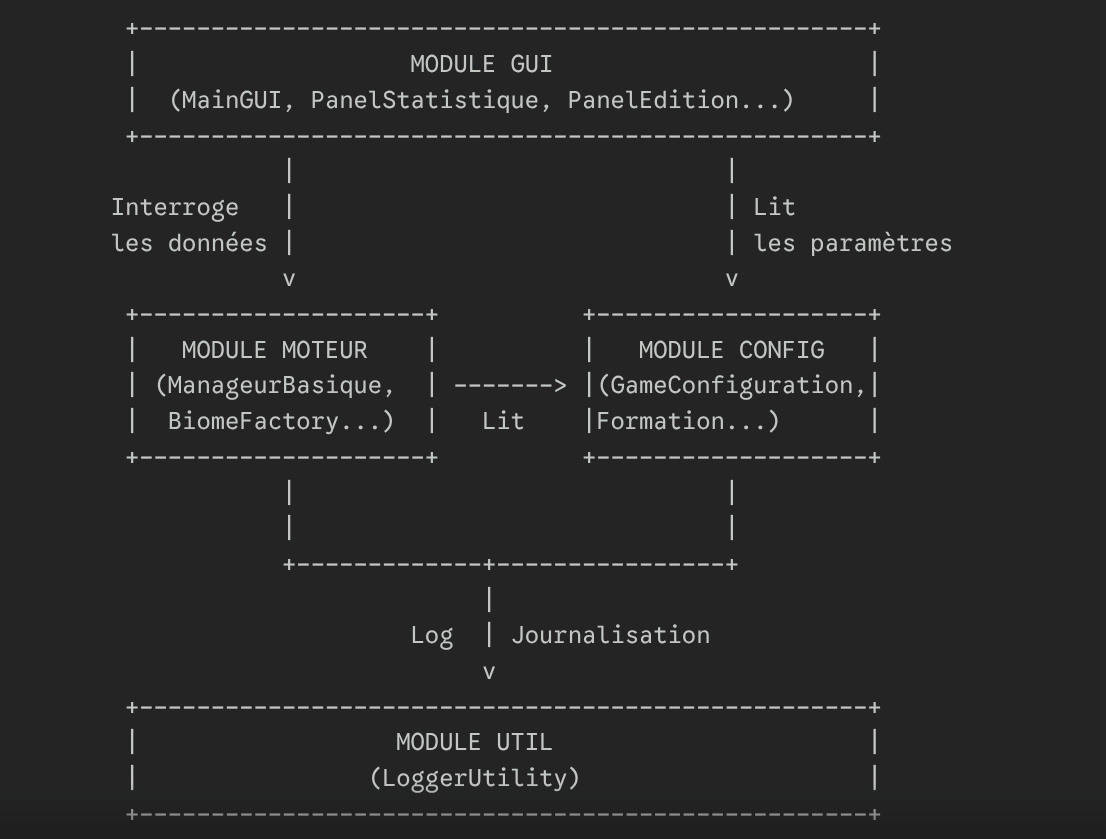
\includegraphics[width=0.85\textwidth]{images/architecture.png}
  \caption{Architecture modulaire de l'application Environnement}
  \label{fig:architecture}
\end{figure}
\needspace{5\baselineskip}
Les quatre modules identifiés dans la figure~\ref{fig:architecture} sont les
suivants.

\begin{itemize}
  \item \textbf{Module \texttt{moteur}}~: constitue le cœur de la simulation. Il
    contient la logique métier~: gestion de la carte, des biomes, des événements
    et des règles de transformation. Ce module est indépendant de l'interface
    graphique et peut fonctionner sans interaction utilisateur.
  \item \textbf{Module \texttt{gui}}~: gère l'interface utilisateur. Il contient
    les classes d'affichage (\texttt{MainGUI}, \texttt{MainDisplayer},
    \texttt{PanelStatistique}, \texttt{PanelTemps}, \texttt{PanelEdition},
    \texttt{TutorielPanel}) et la classe de rendu (\texttt{StrategiePeinture}).
    Ce module dépend du module \texttt{moteur} pour récupérer les données à
    afficher.
  \item \textbf{Module \texttt{config}}~: centralise tous les paramètres~:
    caractéristiques initiales des biomes, effets des événements, seuils de
    transformation et probabilités de génération.
  \item \textbf{Module \texttt{util}}~: regroupe les utilitaires transversaux,
    dont le système de journalisation (\texttt{LoggerUtility}) et la configuration
    Log4j. Il est utilisé par tous les autres modules.
\end{itemize}

Cette séparation en modules garantit que toute modification d'un module n'impacte
  pas les autres, à condition de respecter les interfaces publiques définies. Elle
  facilite également les tests unitaires de chaque composant de manière isolée.

  \paragraph{Positionnement MVC.}
  L'architecture du projet s'articule autour du modèle MVC (Modèle-Vue-Contrôleur).
  Le Modèle (M) correspond au module \texttt{moteur}, qui contient les classes
  \texttt{ManageurBasique}, \texttt{Carte}, \texttt{Biome} et \texttt{Evenement}.
  La Vue (V) est assurée par le module \texttt{gui} via les classes
  \texttt{MainGUI} et \texttt{StrategiePeinture} qui gèrent le rendu graphique.
  Les Contrôleurs (C) sont les Listeners des boutons Swing, qui font le lien entre
  les interactions utilisateur et le moteur de simulation.

% ------------------------------------------------------------
\needspace{15\baselineskip}
\subsection{Classes de données}
\label{subsec:classes_donnees}

Cette sous-section décrit la conception des classes représentant les entités
fondamentales de l'écosystème~: biomes, événements et carte. Elle présente
également les propriétés initiales des biomes, qui constituent un paramètre
central du comportement de la simulation.

\paragraph{Hiérarchie des biomes.}
La classe abstraite \texttt{Biome} constitue la racine de la hiérarchie. Elle
définit les attributs communs à tous les biomes (température, humidité, pollution,
purification, position et bloc associé) ainsi que les méthodes d'accès et de
modification de ces propriétés. Sept sous-classes héritent de \texttt{Biome}~:
\texttt{Foret}, \texttt{Desert}, \texttt{Mer}, \texttt{Montagne}, \texttt{Banquise},
\texttt{Ville} et \texttt{Village}. Chaque sous-classe initialise ses quatre
propriétés avec les valeurs définies dans le module \texttt{config} (constantes de
\texttt{ConfigurationBiome}). Ce couplage faible entre les valeurs de configuration
et les classes concrètes permet de modifier les paramètres de simulation sans
toucher à la logique métier.

\paragraph{Propriétés initiales des biomes.}
Le tableau~\ref{tab:biomes_init} présente les valeurs initiales des quatre
propriétés pour chaque type de biome, telles que définies dans la classe
\texttt{ConfigurationBiome}. Ces valeurs servent de point de départ à chaque
simulation et influencent directement la fréquence et la nature des transformations
déclenchées.

Les propriétés listées dans le tableau~\ref{tab:biomes_init} évoluent sous l'effet
des événements climatiques et peuvent déclencher les transformations automatiques
définies dans le tableau~\ref{tab:transformations}. La Montagne est la seule
exception~: ses propriétés ne peuvent être modifiées par aucune règle ni aucun
événement.

\paragraph{Hiérarchie des événements.}
La classe abstraite \texttt{Evenement} représente la base de tous les phénomènes
météorologiques. Elle contient les attributs communs~: position sur la carte,
direction de déplacement, durée de vie résiduelle et impacts sur les quatre
propriétés des biomes. Deux catégories d'événements héritent de cette classe~:
les événements statiques (\texttt{Meteore}) qui restent à position fixe, et les
événements mobiles (\texttt{Pluie}, \texttt{VentFroid}, \texttt{VentChaud},
\texttt{Pollution}, \texttt{Purification}, \texttt{Orage}, \texttt{Grele},
\texttt{Tornade}, \texttt{PluieBenite}, \texttt{Zephyr}, \texttt{Tonnerre},
\texttt{Smog}, \texttt{NuageToxique}) qui se déplacent d'une case à chaque round.
\needspace{5\baselineskip}
\paragraph{Gestion de la carte.}
La classe \texttt{Carte} gère la grille de simulation. Elle contient un tableau
bidimensionnel d'objets \texttt{Bloc}. Chaque objet \texttt{Bloc} encapsule un
biome et ses coordonnées $(x, y)$. La classe \texttt{Carte} expose des méthodes
pour accéder aux blocs via leurs coordonnées et pour valider la position avant
tout accès, évitant ainsi les accès hors limites.

Le patron Fabrique~\cite{gamma1994design,freeman2004head} est mis en œuvre par les classes
\texttt{BiomeFactory} et \texttt{EvenementFactory}. La \texttt{BiomeFactory}
centralise la création de tous les biomes, permettant d'instancier un biome à
partir de son type sans connaître la classe concrète. La \texttt{EvenementFactory}
crée chaque événement selon une \emph{formation spatiale} précise (unique,
ligne, carré, T, L, diagonale, cercle, croix), définie dans le module
\texttt{config}. Ce patron garantit que l'ajout d'un nouveau type de biome ou
d'événement ne nécessite de modifier que la factory correspondante.

% ------------------------------------------------------------
\subsection{Interface Homme-Machine graphique}
\label{subsec:ihm}

Cette sous-section décrit la conception de l'interface graphique réalisée avec
la bibliothèque Java Swing~\cite{oracle_swing}. Le flux d'ouverture des fenêtres
suit une logique séquentielle~: l'utilisateur commence par le mode édition pour
configurer la carte, puis lance la simulation, ce qui provoque l'affichage de la
fenêtre principale.

\paragraph{Fenêtre d'édition.}
La fenêtre d'édition, implémentée par la classe \texttt{PanelEdition}, constitue le
point d'entrée de l'application. Elle permet à l'utilisateur de configurer la carte
avant le lancement de la simulation. La zone supérieure affiche la grille
(\texttt{MainDisplayer}) où chaque cellule représente un biome. Un panneau
latéral gauche (\texttt{PanelEdition}) donne accès aux sliders de configuration des
probabilités d'événements, organisés par biome source (forêt, désert, mer, ville,
village, banquise). La barre inférieure propose les boutons \textit{Générer Carte}
pour remplir la grille aléatoirement, \textit{Lancer} pour démarrer la
simulation, \textit{Réinitialiser} et \textit{Mettre à zéro} pour restaurer les
valeurs par défaut, ainsi que \textit{Modifier} pour changer manuellement un biome
sélectionné sur la grille. Le mode édition est accessible uniquement avant le
lancement de la simulation ; une fois celle-ci démarrée, la modification
manuelle des cellules est désactivée.

\begin{figure}[htbp]
  \centering
  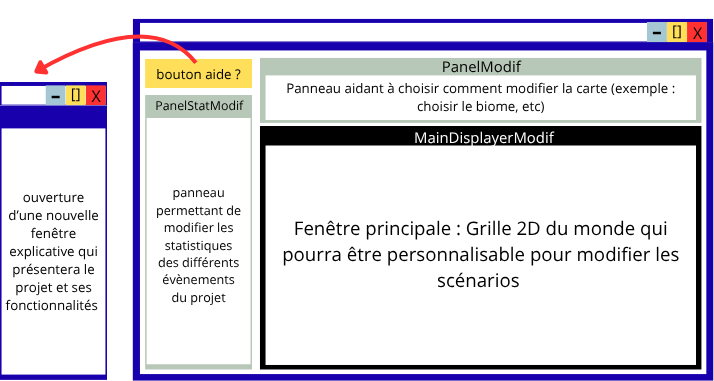
\includegraphics[width=0.9\textwidth]{images/mode_edition.png}
  \caption{Schéma conceptuel de l'interface de configuration initiale}
  \label{fig:schema_edition}
\end{figure}

\needspace{7\baselineskip}
\paragraph{Fenêtre de simulation.}
Lorsque l'utilisateur clique sur le bouton \textit{Lancer}, la fenêtre d'édition
se ferme et la fenêtre principale de simulation s'ouvre. Comme le montre la
figure~\ref{fig:fenetre_simulation}, elle est composée de trois zones
fonctionnelles.

Les trois zones visibles dans la figure~\ref{fig:fenetre_simulation} sont les
suivantes~:

\begin{itemize}
  \item la zone centrale (\texttt{MainDisplayer}) affiche la grille de simulation
    avec les biomes et les événements superposés~;
  \item le panneau latéral droit (\texttt{PanelStatistique}) présente les
    statistiques en temps réel (décompte de chaque type de biome) et les graphiques
    JFreeChart d'évolution des propriétés~;
  \item le panneau inférieur (\texttt{PanelTemps}) regroupe les contrôles de
    simulation (Play, Pause, Vitesse~$\times 2$, Bilan de fin).
\end{itemize}

La structure logique de ces contrôles de pilotage est illustrée dans la
figure~\ref{fig:schema_simulation}.

\begin{figure}[htbp]
  \centering
  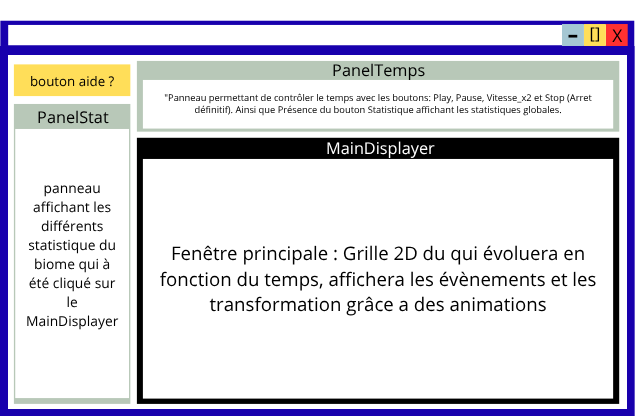
\includegraphics[width=0.85\textwidth]{images/mode_simulation.png}
  \caption{Schéma conceptuel de l'interface de pilotage dynamique}
  \label{fig:schema_simulation}
\end{figure}

\begin{figure}[htbp]
  \centering
  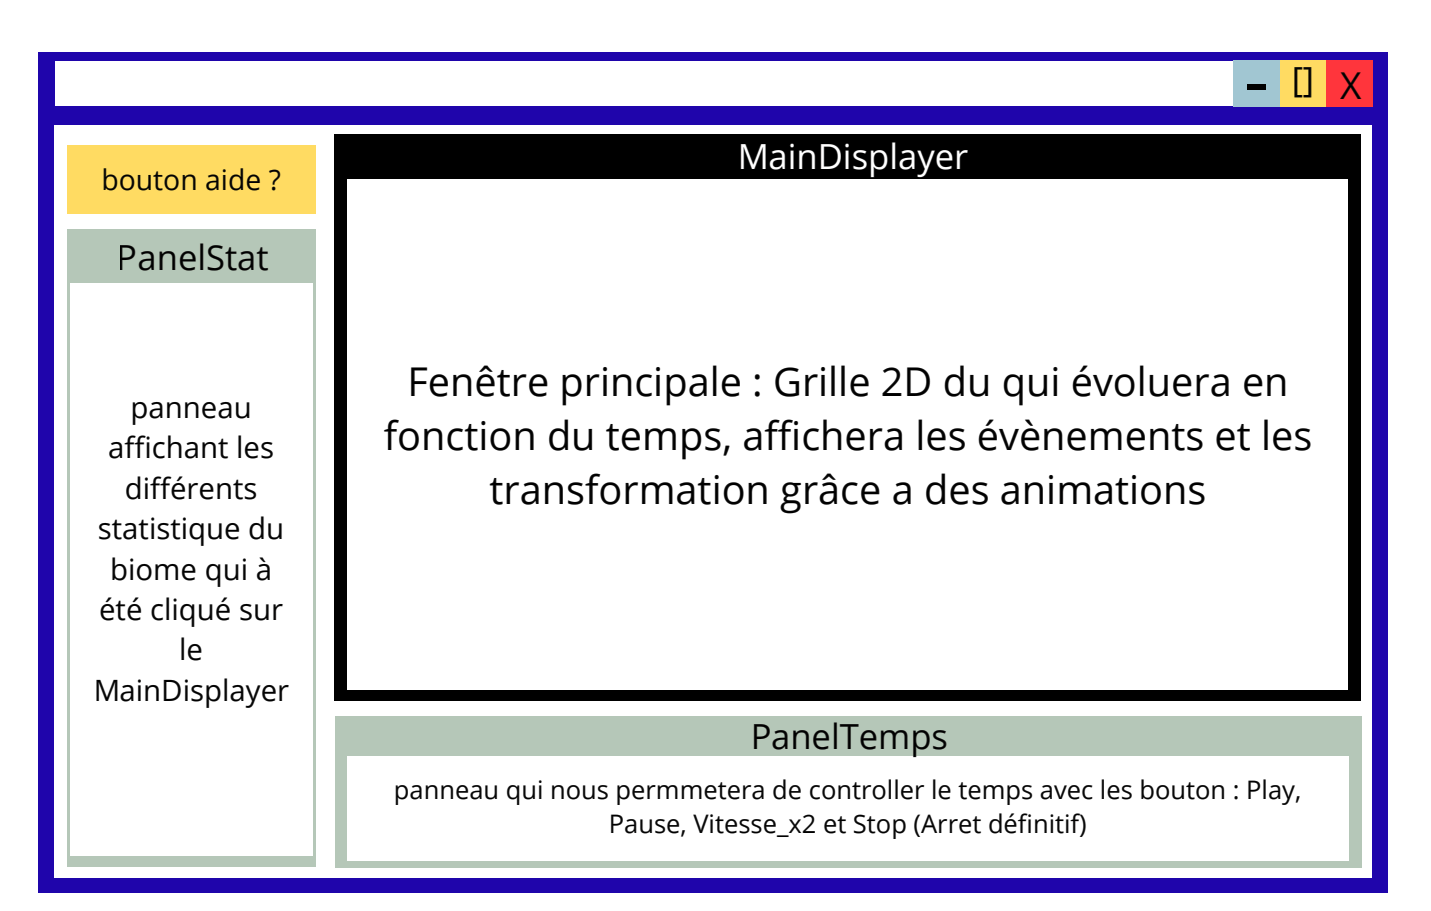
\includegraphics[width=0.9\textwidth]{images/fenetre_simulation.png}
  \caption{Fenêtre principale de simulation avec ses trois zones fonctionnelles}
  \label{fig:fenetre_simulation}
\end{figure}

\needspace{10\baselineskip}
\paragraph{Fenêtre de tutoriel.}
Afin d'améliorer l'accessibilité de l'application, une fenêtre de tutoriel a été
intégrée. Accessible depuis la fenêtre principale via un bouton dédié, elle est
implémentée par la classe \texttt{TutorielPanel} et s'affiche dans une
\texttt{JDialog} modale. Cette fenêtre présente les règles fondamentales de la
simulation~: le rôle de chaque type de biome, le comportement des événements et
la logique des transformations écologiques. L'affichage modal garantit que
l'utilisateur peut consulter ces informations contextuelles sans que la simulation
en cours ne soit interrompue ni fermée.

\begin{figure}[htbp]
  \centering
  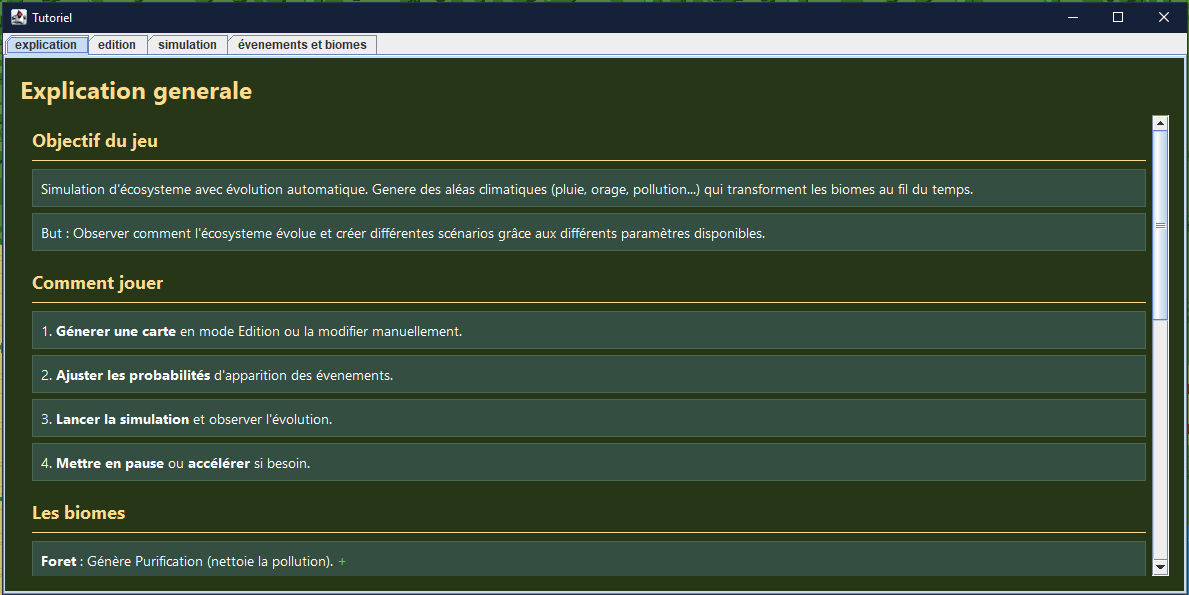
\includegraphics[width=0.9\textwidth]{images/fenetre_aide.png}
  \caption{Fenêtre de tutoriel}
  \label{fig:fenetre_aide}
\end{figure}

\paragraph{Strategy de rendu.}
La classe \texttt{StrategiePeinture} centralise le rendu graphique de l'ensemble
des éléments de la simulation. Chaque méthode \texttt{paintComponent} est
spécialisée pour dessiner un type précis de biome ou d'événement, ce qui permet
d'adapter l'apparence visuelle de chaque élément indépendamment du reste du code
d'affichage. Cette spécialisation facilite l'ajout d'un nouveau rendu graphique
sans modifier les classes de données ni le moteur de simulation.

% ------------------------------------------------------------
\needspace{8\baselineskip}
\subsection{Conception des traitements algorithmiques}
\label{subsec:traitements}

Cette sous-section détaille la logique algorithmique et mathématique du module
\texttt{moteur}. Les formules utilisées pour les transformations, la génération
de la carte et la boucle principale de simulation y sont explicitées.

\paragraph{Formules mathématiques.}
Trois formules régissent le comportement quantitatif de la simulation.

La première formule concerne la \textbf{probabilité de génération d'un événement}.
Pour chaque type d'événement, une probabilité est définie dans la classe
\texttt{ConfigurationCreationEvenement}. Un événement est généré à chaque round
si un nombre aléatoire tiré uniformément est inférieur à cette probabilité~:

\begin{equation}
  \label{eq:proba_generation}
  P(\text{génération}) = p_{\text{configurée}}.
\end{equation}

La formule~\ref{eq:proba_generation} permet de contrôler finement la fréquence
d'apparition de chaque type d'événement.

L'équation~\ref{eq:impact} décrit le \textbf{calcul des impacts sur les propriétés}.
Lorsqu'un événement affecte un biome, ses propriétés sont mises à jour par
addition~:

\begin{equation}
  \label{eq:impact}
  p_{\text{nouvelle}} = p_{\text{actuelle}} + \Delta p_{\text{événement}}.
\end{equation}

L'équation~\ref{eq:bornage} assure le \textbf{bornage des valeurs}. Toutes les propriétés
sont contraintes dans l'intervalle $[0, 100]$ pour garantir la cohérence des
données~:

\begin{equation}
  \label{eq:bornage}
  p_{\text{bornée}} = \max\!\left(0,\; \min\!\left(100,\; p\right)\right).
\end{equation}

En Java, la formule~\ref{eq:bornage} est implémentée via les méthodes
\texttt{Math.max} et \texttt{Math.min}, appliquées systématiquement après chaque
mise à jour de propriété.

\needspace{7\baselineskip}
\paragraph{Algorithme de la boucle de simulation.}
L'algorithme principal est implémenté dans la méthode
\texttt{ManageurBasique.nextRound()}. Il exécute un cycle complet à chaque round
selon la séquence décrite dans le listing~\ref{lst:nextrond}.

\begin{lstlisting}[style=algo, label=lst:nextrond,
    caption={Pseudo-code de la méthode nextRound()}]
ALGORITHME nextRound()
  GENERER nouveaux evenements aleatoires
  POUR CHAQUE evenement mobile FAIRE
    CHOISIR direction aleatoire
    DEPLACER evenement d'une case
    SI deplacement bloque (Montagne) ALORS
      CHOISIR nouvelle direction aleatoire
    FIN SI
    APPLIQUER impacts sur le biome cible
  FIN POUR CHAQUE
  POUR CHAQUE biome de la carte FAIRE
    EVALUER toutes les regles de transformation
    SI conditions d'une regle remplies ALORS
      TRANSFORMER biome selon la regle
    FIN SI
  FIN POUR CHAQUE
FIN ALGORITHME
\end{lstlisting}

L'algorithme présenté dans le listing~\ref{lst:nextrond} garantit que les quatre
étapes de la simulation sont exécutées dans un ordre déterministe à chaque round.

\needspace{20\baselineskip}
\paragraph{Algorithme de génération de la carte.}
La génération cohérente des biomes est implémentée dans
\texttt{BiomeFactory.creerBiomesCoherents()}. Cet algorithme crée une distribution
géographiquement plausible, avec des masses d'eau, des zones désertiques et des
zones urbaines, comme le présente le listing~\ref{lst:gencarte}.

\begin{lstlisting}[style=algo, label=lst:gencarte,
    caption={Pseudo-code de la génération cohérente de la carte}]
ALGORITHME creerBiomesCoherents()
  GENERER masse d'eau (forme aleatoire : coin, haut ou milieu)
  POUR CHAQUE case de la grille FAIRE
    CALCULER distance a la masse d'eau par BFS
  FIN POUR
  POUR CHAQUE case proche de l'eau ET loin d'une zone desertique FAIRE
    AFFECTER biome Village
  FIN POUR
  POUR CHAQUE case loin de l'eau ET en zone desertique FAIRE
    AFFECTER biome Desert
  FIN POUR
  POUR CHAQUE case en zone urbaine FAIRE
    AFFECTER biome Ville
  FIN POUR
  RETOURNER carte avec biomes coherents
FIN ALGORITHME
\end{lstlisting}

Les distances à la masse d'eau utilisées dans le listing~\ref{lst:gencarte} sont
calculées par propagation BFS (\textit{Breadth-First Search}), algorithme de
parcours en largeur~\cite{cormen2009intro}, pour déterminer les zones propices à
chaque type de biome.

\paragraph{Règles de transformation écologique.}
Six règles implémentent l'interface \texttt{RegleTransformation}. Chaque règle
évalue les propriétés d'un biome (température, humidité, pollution, purification)
et retourne un nouveau biome si les conditions définies dans le
tableau~\ref{tab:transformations} sont satisfaites. Les règles implémentées
sont~: Inondation, Glaciation, Désertification, Forestation, Civilisation et
Densification. Chaque règle encapsule ses conditions dans une méthode
\texttt{appliquer(Biome b)} qui retourne le biome cible ou \texttt{null} si les
conditions ne sont pas réunies~; le moteur applique simplement le premier résultat
non nul.

\needspace{7\baselineskip}
\paragraph{Génération d'événements depuis les biomes.}
La classe \texttt{EvenementFactory} crée des événements selon des probabilités
configurées dans \texttt{ConfigurationCreationEvenement}. Le patron Visiteur est
incarné par la classe \texttt{GenerateurEvenementVisitor}, qui parcourt la carte et
génère des événements supplémentaires depuis certains biomes (par exemple, un biome
Mer génère périodiquement un événement Pluie selon son identité propre). Les
probabilités de génération et les formations spatiales des événements sont
entièrement définies dans le module \texttt{config}, ce qui permet de les modifier
sans recompiler la logique métier.

\paragraph{Système de journalisation.}
Le système repose sur la bibliothèque Log4j~\cite{apache_log4j}. La classe
utilitaire \texttt{LoggerUtility} fournit un accès centralisé au logger de
l'application~; elle est conçue pour être utilisée statiquement depuis n'importe
quel module. Les journaux sont émis aux niveaux \texttt{DEBUG} et \texttt{INFO},
et écrits simultanément vers la console et vers le fichier
\texttt{src/logs/simulation.log}. Les actions journalisées incluent notamment le
démarrage et la fin de chaque round, les déplacements d'événements, les
transformations de biomes et les anomalies détectées lors de l'exécution.

\paragraph{Gestion des statistiques.}
L'affichage des statistiques en temps réel repose sur la bibliothèque
JFreeChart~\cite{jfreechart}. Les données collectées à chaque round (répartition
des biomes, évolution des propriétés moyennes) sont injectées dans des
\texttt{XYSeriesCollection} qui alimentent les graphiques du
\texttt{PanelStatistique}. Ce mécanisme permet de visualiser l'évolution temporelle
de l'écosystème avec une précision et une lisibilité supérieures aux représentations
visuelles purement symboliques.

% ============================================================
%  MANUEL UTILISATEUR — manuel.tex
% ============================================================
\section{Manuel d'installation et d'utilisation}
\label{sec:manuel}

Cette section constitue le guide de référence destiné à toute personne souhaitant
installer, compiler et utiliser l'application Environnement. Les instructions
sont organisées de façon séquentielle~: prérequis, procédure de compilation,
lancement de l'application, puis guide d'utilisation de l'interface graphique.

% ------------------------------------------------------------
\subsection{Prérequis et environnement technique}
\label{subsec:prerequis}

Avant de procéder à l'exécution, il est nécessaire de vérifier que le Java
Development Kit (JDK)~8 ainsi que les bibliothèques listées dans le
tableau~\ref{tab:prerequis} sont présents sur la machine hôte. Un environnement
de développement intégré est également requis pour compiler le projet~; Eclipse
est recommandé car il a été utilisé lors du développement et garantit une
compatibilité optimale avec la configuration du projet.

\begin{table}[H]
  \centering
  \caption{Bibliothèques prérequises pour le bon fonctionnement de l'application}
  \label{tab:prerequis}
  \begin{tabular}{ll}
    \toprule
    \textbf{Bibliothèque} & \textbf{Rôle} \\
    \midrule
    jcommon       & Utilitaires communs JFreeChart \\
    hamcrest-core & Assertions pour les tests unitaires \\
    jfreechart    & Génération de graphiques 2D \\
    jfreesvg      & Export des graphiques au format SVG \\
    junit         & Framework de tests unitaires \\
    log4j         & Journalisation applicative \\
    swtgraphics2d & Pont entre SWT et Graphics2D \\
    \bottomrule
  \end{tabular}
\end{table}

L'application est compatible avec les systèmes d'exploitation Windows~10 ou
ultérieur, GNU/Linux (distributions Debian et dérivées) et macOS~12 ou ultérieur.
Une résolution d'écran d'au moins 1920\,$\times$\,1080~pixels est recommandée pour
un affichage optimal de l'interface graphique.

% ------------------------------------------------------------
\subsection{Récupération et compilation du projet}
\label{subsec:compilation}

La récupération du code source s'effectue via Git, puis la compilation est
réalisée depuis Eclipse.

\paragraph{Récupération du code source.}
La méthode recommandée est d'utiliser GitHub Desktop, qui simplifie la gestion du
dépôt. Après installation, le dépôt se clone via
\textit{File > Clone repository} en renseignant l'URL du projet~:

\begin{lstlisting}[style=java, language=bash, label=lst:clone,
    caption={Clonage du dépôt via GitHub Desktop}]
File > Clone repository > URL > coller l'URL du depot > Clone
\end{lstlisting}

Pour les utilisateurs ne souhaitant pas installer GitHub Desktop, il est possible
de télécharger le projet directement depuis l'interface web de GitHub~:

\begin{lstlisting}[style=java, language=bash, label=lst:zip,
    caption={Téléchargement du projet via l'interface web}]
Code > Download ZIP > extraire l'archive sur la machine locale
\end{lstlisting}

\paragraph{Compilation avec Eclipse.}
Une fois le projet récupéré, il convient de l'importer dans Eclipse en
suivant le chemin~:

\begin{lstlisting}[style=java, language=bash, label=lst:import,
    caption={Import du projet dans Eclipse}]
File > Import > Existing Projects into Workspace
  > selectionner le repertoire racine
\end{lstlisting}

Les bibliothèques listées dans le tableau~\ref{tab:prerequis} doivent ensuite être
ajoutées au build path~:

\begin{lstlisting}[style=java, language=bash, label=lst:buildpath,
    caption={Ajout des bibliothèques au build path}]
Project > Properties > Java Build Path > Add External JARs
\end{lstlisting}

La compilation s'effectue ensuite automatiquement à chaque sauvegarde si l'option
\textit{Build Automatically} est activée dans le menu \textit{Project}.

% ------------------------------------------------------------
\subsection{Lancement et utilisation de l'application}
\label{subsec:lancement}

Une fois le projet compilé conformément à la section~\ref{subsec:compilation},
l'application se lance depuis Eclipse en exécutant directement le fichier
\texttt{Environnement.java} via le menu~:

\begin{lstlisting}[style=java, language=bash, label=lst:run,
    caption={Lancement de l'application depuis Eclipse}]
Run > Run As > Java Application
\end{lstlisting}

Il est également possible de lancer l'application depuis un terminal si un fichier
\texttt{.jar} exécutable a été exporté au préalable via
\textit{File > Export > Runnable JAR file}~:

\begin{lstlisting}[style=java, language=bash, label=lst:runjar,
    caption={Lancement de l'application depuis un terminal}]
java -jar /chemin/vers/Environnement.jar
\end{lstlisting}

L'interface graphique s'ouvre automatiquement après quelques instants.

\paragraph{Étape 1 — Mode édition.}
Au lancement, la fenêtre d'édition s'affiche. Elle permet de configurer manuellement
la carte avant de démarrer la simulation. La figure~\ref{fig:manuel_edition}
présente l'aspect de cette fenêtre avec ses différentes zones de contrôle.

\begin{figure}[H]
  \centering
  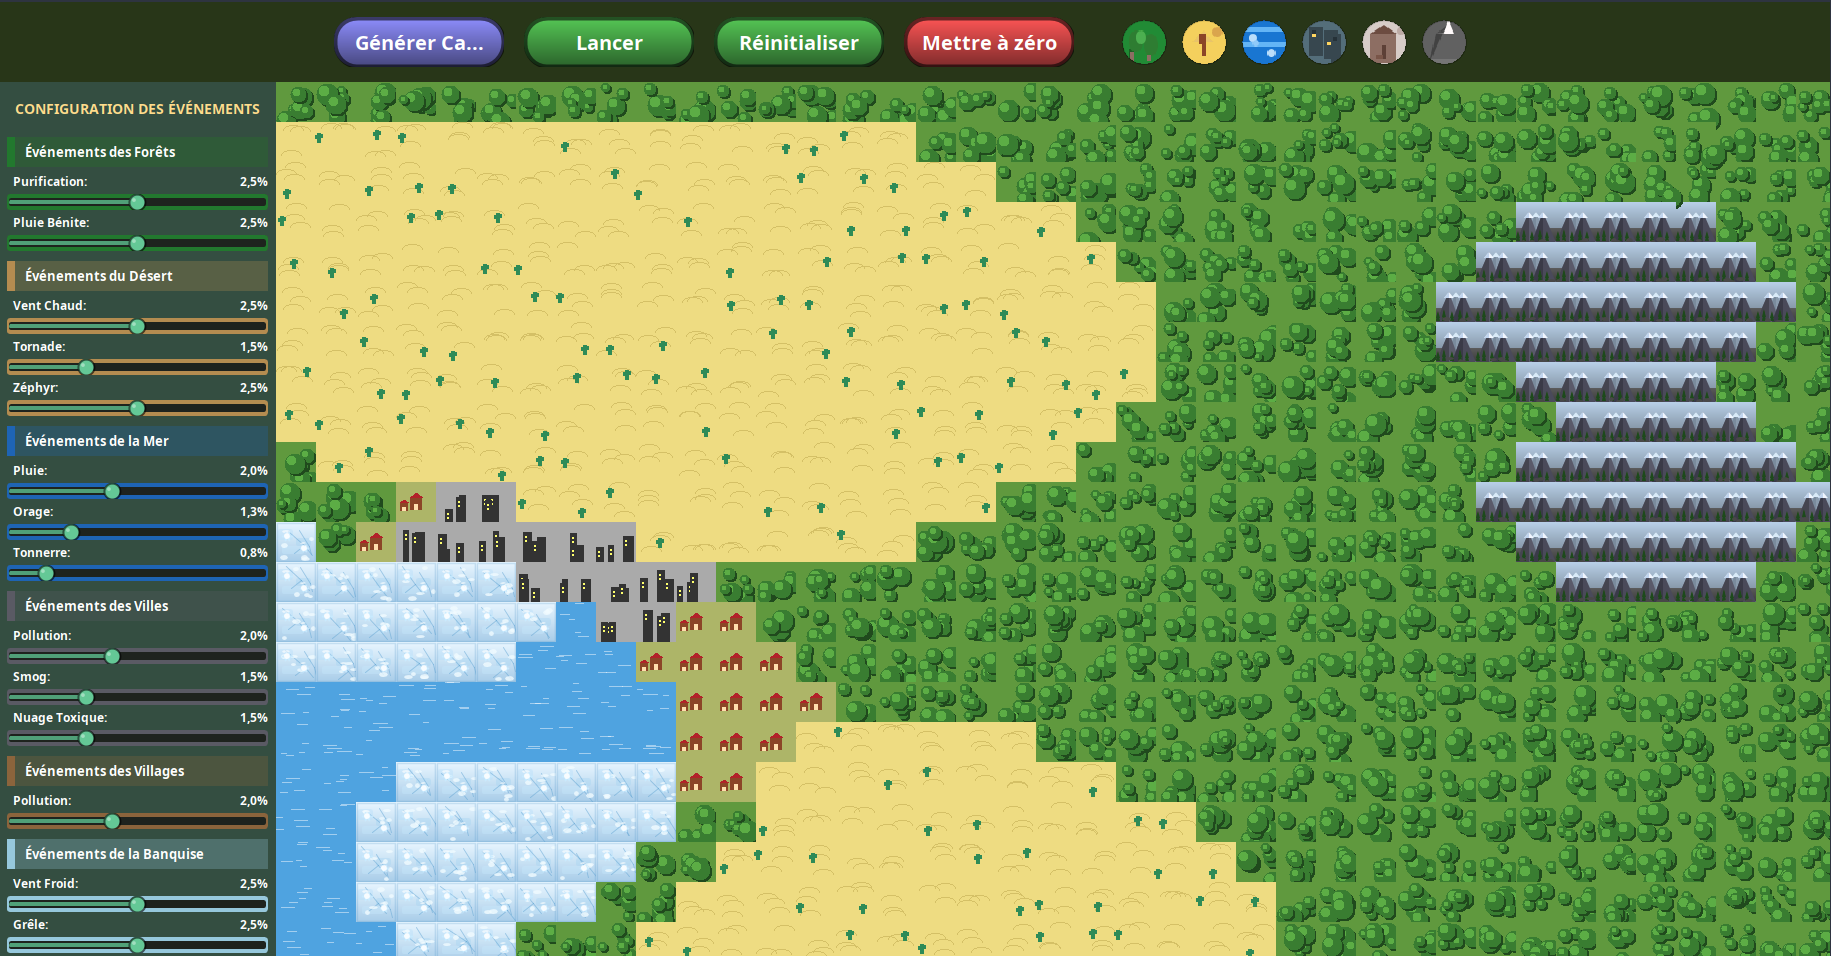
\includegraphics[width=0.85\textwidth]{images/image_edition}
  \caption{Fenêtre d'édition~: configuration de la carte et des probabilités
           d'événements}
  \label{fig:manuel_edition}
\end{figure}

Comme on peut le constater sur la figure~\ref{fig:manuel_edition}, les opérations
disponibles dans cette fenêtre sont les suivantes~:

\begin{itemize}
  \item modifier les probabilités qu'un événement survienne via le menu de gauche~;
  \item réinitialiser ou remettre à zéro les probabilités des événements avec les
    boutons \textit{Réinitialiser} ou \textit{Mettre à zéro}~;
  \item cliquer sur un biome pour ensuite changer sa nature avec le bouton
    \textit{Modifier}~;
  \item utiliser le bouton \textit{Génération aléatoire} pour remplir
    automatiquement la carte avec une distribution pseudo-aléatoire de biomes.
\end{itemize}

\paragraph{Étape 2 — Lancement de la simulation.}
Le bouton \textit{Lancer la simulation} ferme la fenêtre d'édition et ouvre la
fenêtre principale de simulation. La simulation débute automatiquement dès
l'ouverture de cette fenêtre.

\paragraph{Étape 3 — Contrôle de la simulation.}
Les contrôles disponibles dans le panneau inférieur (\texttt{PanelTemps})
permettent de piloter l'exécution. Le tableau~\ref{tab:controles} décrit chaque
bouton et son effet.

\begin{table}[H]
  \centering
  \caption{Contrôles de la simulation et leurs effets}
  \label{tab:controles}
  \begin{tabular}{ll}
    \toprule
    \textbf{Contrôle} & \textbf{Effet} \\
    \midrule
    \textit{Play}              & Démarre ou reprend la simulation après une pause \\
    \textit{Pause}             & Suspend l'exécution à la fin du round en cours \\
    \textit{Vitesse $\times 2$} & Double la cadence d'enchaînement des rounds \\
    \textit{Bilan de fin}      & Affiche un récapitulatif statistique de la simulation \\
    \textit{Statistiques}      & Ouvre la fenêtre d'analyse détaillée en temps réel \\
    \textit{Tutoriel}          & Ouvre la fenêtre d'aide et de présentation des règles \\
    \bottomrule
  \end{tabular}
\end{table}

\paragraph{Étape 4 — Lecture des statistiques.}
La figure~\ref{fig:manuel_simulation} illustre l'interface principale lors d'une
session en cours, avec ses trois zones fonctionnelles~: la grille centrale de
simulation, le panneau de statistiques et les contrôles de pilotage.

\begin{figure}[H]
  \centering
  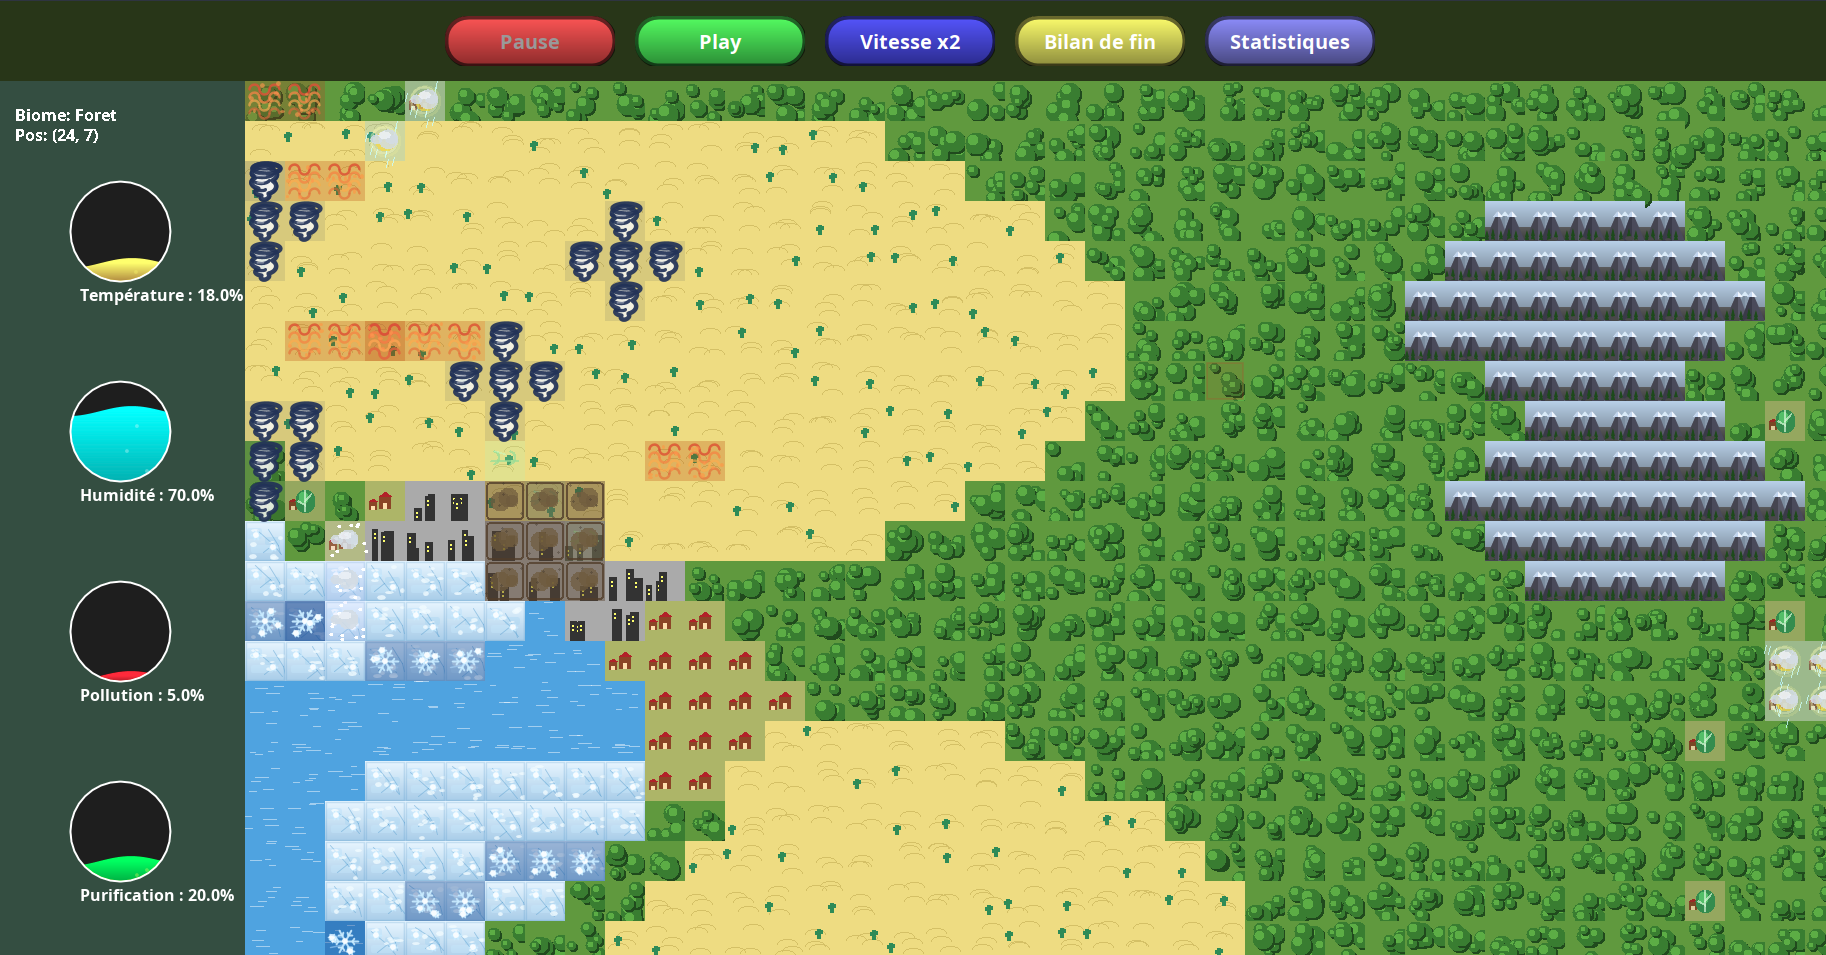
\includegraphics[width=0.9\textwidth]{images/image_simulation}
  \caption{Fenêtre principale de simulation~: grille, statistiques JFreeChart et
           contrôles}
  \label{fig:manuel_simulation}
\end{figure}

Tel qu'illustré dans la figure~\ref{fig:manuel_simulation}, le panneau latéral
droit affiche les statistiques en temps réel ainsi que les graphiques d'évolution
des propriétés générés par JFreeChart. En cliquant sur un biome de la grille
centrale, ses propriétés détaillées (température, humidité, pollution,
purification) s'affichent dans ce même panneau. La fenêtre \textit{Statistiques},
accessible depuis le tableau~\ref{tab:controles}, présente une analyse agrégée
de l'ensemble de la simulation sous forme graphique.

\paragraph{Consultation des journaux d'exécution.}
En cas d'anomalie ou à des fins d'analyse, les journaux de la session en cours sont
accessibles dans le fichier \texttt{src/logs/simulation.log}. Chaque entrée de
journal comporte un horodatage, un niveau de sévérité (\texttt{INFO} ou
\texttt{DEBUG}) et un message descriptif de l'action enregistrée.

% ============================================================
%  DÉROULEMENT DU PROJET — deroulement.tex
% ============================================================
\section{Déroulement du projet}
\label{sec:deroulement}

Cette section retrace l'organisation du travail d'équipe et les étapes successives
ayant conduit à l'application décrite dans la section~\ref{sec:realisation}. Elle
présente la méthode de collaboration adoptée, la répartition des responsabilités,
les outils de développement utilisés, et les principaux obstacles surmontés au
cours du projet.

% ------------------------------------------------------------
\subsection{Organisation et répartition du travail}
\label{subsec:organisation_travail}

L'équipe est composée de trois développeurs~: \textsc{Feraoun} Mohamed~Amine,
\textsc{Anurajan} Thenuxshan et \textsc{Ouardani} Nidhal. Afin de tirer parti de
la modularité de l'architecture décrite à la section~\ref{subsec:archi_globale},
la répartition des tâches a suivi un découpage fonctionnel cohérent avec les
quatre modules du projet.

\paragraph{Répartition du travail.}
Feraoun Mohamed Amine a conçu l'architecture modulaire et le cœur du moteur de
simulation (classes Carte, ManageurBasique, règles de transformation). Il a
réalisé les tests unitaires et rédigé la première partie du rapport.

Ouardani Nidhal a mis en place le système de journalisation Log4j et a développé
l'algorithme de génération cohérente de la carte et la logique de déplacement
des événements mobiles. Il a contribué à la rédaction de la deuxième partie du
rapport.

Anurajan Thenuxshan a implémenté le module de configuration et la fenêtre
d'édition (PanelEdition), assurant l'interface de paramétrage des événements. Il a
apporté un support technique sur les composantes graphiques et participé aux tests
d'intégration.

Cette répartition n'a pas été strictement cloisonnée~: des révisions croisées du
code ont été systématiquement organisées pour garantir la cohérence globale du
projet et mutualiser les connaissances techniques entre les membres de l'équipe.

\paragraph{Méthode de travail collaborative.}
Un dépôt Git commun~\cite{chacon2014pro} (lien~: \url{https://github.com/MLX-JAY/Environnement}) a servi de base au travail collaboratif.
Chaque fonctionnalité a été développée sur une branche dédiée avant d'être
fusionnée vers la branche principale après revue de code. Des réunions d'équipe
hebdomadaires ont permis de synchroniser les avancées, d'identifier les dépendances
entre modules et d'ajuster le planning.

% ------------------------------------------------------------
\subsection{Phases de développement}
\label{subsec:phases}

Le développement s'est articulé en quatre phases successives dont les jalons sont
présentés dans le tableau~\ref{tab:planning}.

\begin{table}[htbp]
  \centering
  \caption{Phases de développement et jalons du projet}
  \label{tab:planning}
  \begin{tabular}{cl>{\raggedright\arraybackslash}p{8cm}}
    \toprule
    \textbf{Phase} & \textbf{Période} & \textbf{Objectifs et livrables} \\
    \midrule
    1 & Semaines 1--2  & Analyse des besoins, conception de l'architecture,
                         mise en place de l'environnement de développement
                         et du dépôt Git \\[0.4em]
    2 & Semaines 3--5  & Implémentation des classes de données (biomes,
                         événements, carte), module \texttt{config},
                         premières règles de transformation \\[0.4em]
    3 & Semaines 6--8  & Développement du moteur de simulation
                         (\texttt{ManageurBasique}), intégration des factories,
                         réalisation de l'interface graphique \\[0.4em]
    4 & Semaines 9--10 & Finalisation des différents concepts du projet
                         (comme le mode édition), corrections des anomalies
                         et bilan de fin ; rédaction du rapport \\
    \bottomrule
  \end{tabular}
\end{table}

% ------------------------------------------------------------
\subsection{Difficultés rencontrées et solutions adoptées}
\label{subsec:difficultes}

Plusieurs difficultés techniques ont été rencontrées au cours du développement.
Elles sont décrites dans la section~\ref{subsec:difficultes} sous la forme d'un couple problème/solution afin
d'en faciliter la compréhension.

\paragraph{Les statistiques.}
\textbf{Problème.}
Une première version des statistiques reposait sur des bulles visuelles se
remplissant proportionnellement à l'état du monde. Cette représentation s'est
révélée imprécise et insuffisante pour suivre l'évolution quantitative de
l'écosystème au fil des rounds.

\textbf{Solution.}
La bibliothèque JFreeChart a été intégrée pour remplacer ce dispositif. Elle
permet d'afficher des graphiques en courbes clairs alimentés en temps réel par les
données de simulation, offrant une lecture précise et rigoureuse des propriétés
des biomes au fil du temps.

\paragraph{Les transformations écologiques.}
\textbf{Problème.}
La gestion dynamique des transformations de biomes s'est avérée complexe à
implémenter~: un premier prototype fondé sur des conditions imbriquées dans le
\texttt{ManageurBasique} était difficile à maintenir et ne tenait pas compte des
spécificités de chaque biome.

\textbf{Solution.}
Un système de règles de transformation a été créé, matérialisé par l'interface
\texttt{RegleTransformation}. Chaque règle est liée aux statistiques propres du
biome concerné et encapsule sa logique de manière autonome. Le moteur se contente
d'itérer sur la liste des règles, ce qui rend l'ensemble extensible et maintenable.

\paragraph{Dynamique des biomes.}
\textbf{Problème.}
Dans une version initiale, la seule différence entre les biomes était d'ordre
visuel (couleur et texture). Tous les biomes recevaient les mêmes types
d'événements, ce qui rendait la simulation peu réaliste et les identités de biomes
interchangeables.

\textbf{Solution.}
Le patron Visiteur (\texttt{GenerateurEvenementVisitor}) a été mis en place pour
que les événements générés dépendent du type de biome visité. Un biome Mer génère
ainsi des événements de type Pluie, tandis qu'un biome Désert favorise des
événements de Zéphyr ou de Tornade. Cette logique renforce l'identité unique de
chaque biome.

\paragraph{Création des événements.}
\textbf{Problème.}
L'apparition d'un événement sur une seule case était peu lisible et manquait de
cohérence visuelle. Un événement de type Orage occupant une cellule unique avait le
même impact visuel qu'une simple Pluie, rendant la lecture de la grille confuse.

\textbf{Solution.}
Un système de formations spatiales a été implémenté directement dans
l'\texttt{EvenementFactory}~: chaque événement est désormais créé selon une
formation géométrique définie (ligne, carré, croix, etc.), via des méthodes de
création dédiées. Ce mécanisme apporte un boost visuel et logique significatif~:
chaque type d'événement possède une empreinte reconnaissable sur la grille, ce qui
renforce la cohérence globale de l'interface.

% ============================================================
%  CONCLUSION — conclusion.tex
% ============================================================
\section{Conclusion et perspectives}
\label{sec:conclusion}

Ce rapport a présenté la conception et l'implémentation du projet Environnement,
un simulateur d'écosystème dynamique développé en Java~8 dans le cadre du cours
de Génie Logiciel et Conception. L'application constitue un système complet et
fonctionnel, capable de simuler l'évolution de biomes soumis à des événements
météorologiques variés et gouvernés par des règles de transformation écologique.

\subsection{Bilan du travail réalisé}
\label{subsec:bilan}

L'ensemble des fonctionnalités définies dans la section~\ref{sec:specification}
a été implémenté. Les sept types de biomes sont modélisés avec leurs propriétés
initiales et leur comportement propre. Les treize événements météorologiques,
statiques et mobiles, sont générés selon des formations spatiales distinctes,
déplacés et appliqués conformément aux spécifications. Les six règles de
transformation écologique évaluent correctement les propriétés des biomes à chaque
round et déclenchent les transformations attendues, telles que définies dans le
tableau~\ref{tab:transformations}. Enfin, l'interface graphique permet de
visualiser la simulation en temps réel et d'en contrôler le déroulement de manière
interactive.

Sur le plan de la conception logicielle, l'architecture modulaire à quatre modules
(\texttt{moteur}, \texttt{gui}, \texttt{config}, \texttt{util}) a démontré son
efficacité~: elle a permis un développement en parallèle, facilité les tests
d'intégration et rendu les corrections d'anomalies plus rapides à localiser. Les
patrons de conception mis en œuvre (Fabrique, Visiteur, programmation par
interfaces) ont contribué à la maintenabilité et à l'extensibilité du code, deux
critères fondamentaux identifiés dans la section~\ref{subsec:enjeux}. L'intégration
de JFreeChart a apporté une valeur analytique concrète à l'application, en
remplaçant des représentations visuelles imprécises par des graphiques rigoureux.

Le travail en équipe de trois développeurs, organisé autour du dépôt Git et de
réunions de synchronisation hebdomadaires, s'est déroulé de manière productive.
La répartition initiale des responsabilités par module, décrite dans la
section~\ref{subsec:organisation_travail}, a limité les conflits de fusion tout
en favorisant la cohésion globale du projet.

\subsection{Perspectives d'amélioration}
\label{subsec:perspectives}

Plusieurs axes d'amélioration ont été identifiés à l'issue du développement.

Le premier axe concerne la \textbf{persistance des données}. L'implémentation d'un
mécanisme de sérialisation au format JSON ou XML permettrait de sauvegarder et de
recharger l'état complet d'une simulation. Cette fonctionnalité rendrait
l'application utilisable dans un contexte pédagogique où les séances sont
fragmentées.

Le deuxième axe porte sur l'\textbf{extensibilité dynamique}. Permettre le
chargement de nouveaux types de biomes ou de nouvelles règles de transformation à
partir de fichiers de configuration externes, sans recompilation, constituerait
une amélioration architecturale significative. Un mécanisme de plugin fondé sur
l'API \textit{Service Loader} de Java serait une solution
adaptée à cette évolution.

Le troisième axe vise l'\textbf{amélioration de l'interface graphique}. Une
refonte vers une mise en page fluide et redimensionnable, recourant par exemple à
la bibliothèque JavaFX, permettrait de lever la contrainte de résolution fixe
identifiée dans la section~\ref{subsec:notions_base}. Cette refonte améliorerait
également l'expérience utilisateur sur les écrans de petite taille.

Enfin, un quatrième axe envisage l'\textbf{enrichissement du modèle de simulation}.
L'introduction de chaînes alimentaires entre espèces animales virtuelles peuplant
les biomes, ou la modélisation de phénomènes climatiques globaux (cycles
hydrologiques, effet de serre simplifié), accroîtrait considérablement le réalisme
et la valeur pédagogique du simulateur.

Ces perspectives confirment que le projet Environnement, dans son état actuel,
constitue une base solide et extensible sur laquelle des développements futurs
peuvent s'appuyer.


% --- Bibliographie (BibTeX) ---
\bibliographystyle{alpha}
\bibliography{references}

% ============================================================
\end{document}
% ============================================================
